\subsection{Visual Motor Deficit}
Visual motor deficit, also known as visual-motor integration difficulty, refers to a condition that impacts a child's ability to coordinate visual perception with motor skills. Individuals with visual motor deficits may experience challenges in tasks requiring hand-eye coordination, spatial awareness, and fine motor control. To develop interventions tailored to the needs of children with visual motor deficits, it is important to understand their unique user profile. This includes identifying their specific goals, psychographics, problems, characteristics, and needs related to visual-motor integration and motor coordination.

\begin{figure}[H]
    \centering
    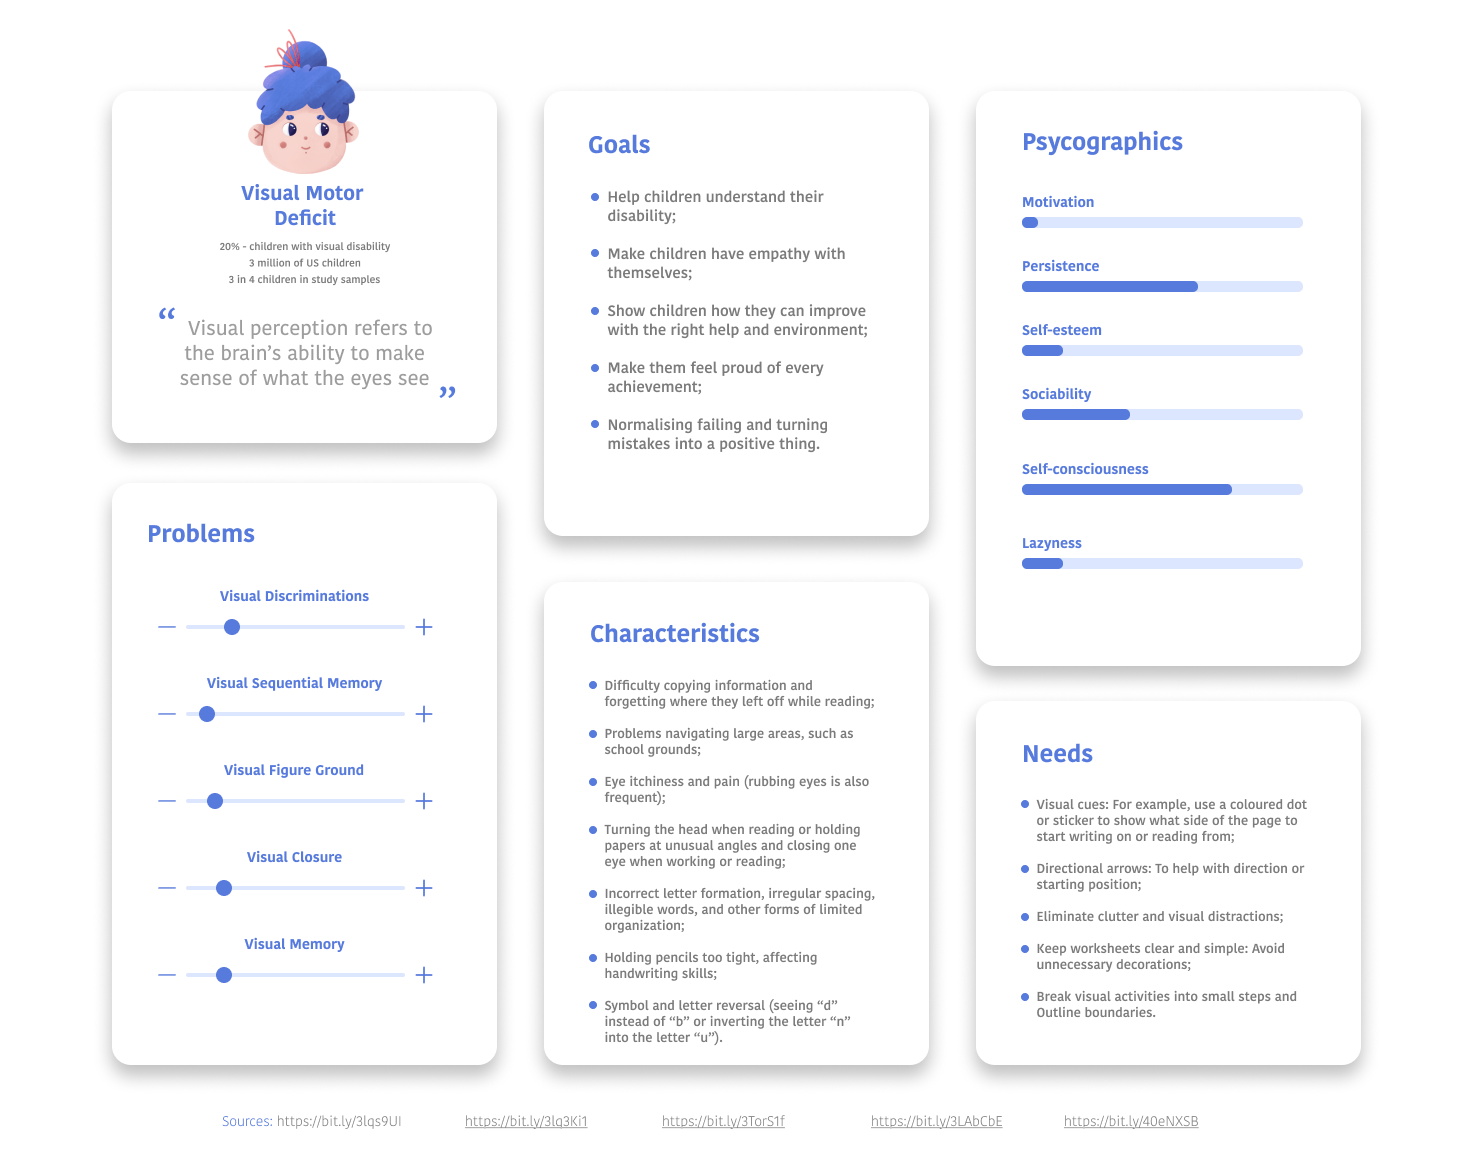
\includegraphics[width=0.8\linewidth]{Chapters/figma/Visual Motor Deficit.png}
    \caption{Visual Motor Deficit User Profile}
    \label{fig:VMDUserProfile}
\end{figure}

\paragraph{Goals}
\begin{itemize}
    \item Helping children understand their disability and fostering self-empathy \cite{PorterAcademy}.
    \item Demonstrating how improvement is achievable with appropriate support and an enabling environment \cite{ScienceDaily}.
    \item Cultivating a sense of pride in every achievement, no matter how small \cite{ChildDevelopment}.
    \item Promoting a positive mindset towards failure, viewing mistakes as opportunities for growth \cite{Speechify}.
\end{itemize}

\paragraph{Psycographics}
\begin{itemize}
    \item Low motivation and self-esteem due to persistent challenges \cite{ChildDevelopment}.
    \item High levels of persistence, showing determination to overcome difficulties \cite{Speechify}.
    \item Average sociability, seeking opportunities for interaction with peers \cite{PorterAcademy}.
    \item Heightened self-consciousness about their motor skills \cite{Speechify}.
    \item Low levels of laziness, indicating a willingness to invest effort in learning and development \cite{PorterAcademy}.
\end{itemize}

\paragraph{Problems}
\begin{itemize}
    \item \textbf{Visual discriminations}: Difficulty distinguishing and recognizing visual details accurately \cite{ChildDevelopment}.
    \item \textbf{Visual sequential memory}: Struggles in remembering and reproducing visual sequences in the correct order \cite{PorterAcademy}.
    \item \textbf{Visual figure-ground}: Difficulty differentiating foreground from background in visual stimuli \cite{ScienceDaily}.
    \item \textbf{Visual closure}: Challenges in perceiving complete images or letters when parts are missing \cite{Speechify}.
    \item \textbf{Visual memory}: Difficulty retaining and recalling visual information accurately \cite{PorterAcademy}.
\end{itemize}

\paragraph{Characteristics}
\begin{itemize}
    \item Difficulty copying information accurately and maintaining their place while reading \cite{Speechify}.
    \item Challenges in navigating large areas and perceiving spatial relationships \cite{PorterAcademy}.
    \item Frequent eye itchiness and pain, leading to rubbing of the eyes \cite{ChildDevelopment}.
    \item Unusual head movements or holding papers at atypical angles while reading or working \cite{Speechify}.
    \item Poor letter formation, irregular spacing, and illegible handwriting \cite{PorterAcademy}.
    \item Excessive grip pressure on pencils, impacting handwriting skills \cite{ScienceDaily}.
    \item Reversal of symbols and letters, such as mistaking ''d'' for ''b'' or inverting the letter ''n'' into ''u'' \cite{ChildDevelopment}.
\end{itemize}

\paragraph{Needs}
\begin{itemize}
    \item \textbf{Visual cues}: Incorporating visual aids, such as colored dots or stickers, to signal the starting point for writing or reading \cite{PorterAcademy}.
    \item \textbf{Directional arrows}: Providing clear visual cues to assist with direction and starting positions \cite{Speechify}.
    \item \textbf{Minimizing clutter and distractions}: Creating organized and uncluttered learning environments to enhance focus and concentration \cite{ChildDevelopment}.
    \item \textbf{Simplifying worksheets}: Presenting worksheets with clear, straightforward designs and avoiding unnecessary decorations \cite{Speechify}.
    \item \textbf{Breaking activities into small steps}: Breaking down visual tasks into manageable steps to facilitate understanding and completion \cite{ScienceDaily}.
    \item \textbf{Outlining boundaries}: Using visual cues, such as borders or highlighting, to delineate boundaries within worksheets or assignments \cite{PorterAcademy}.
\end{itemize}
